\documentclass[12pt,a4paper]{report}
\usepackage[portuguese]{babel}
\usepackage[utf8]{inputenc}
\usepackage{xcolor}
\usepackage{graphicx}
\usepackage[pdftex]{hyperref}
\usepackage{titling}
\usepackage{amsmath}

\setlength{\droptitle}{-2cm}

\title{Projeto de Processamento de Linguagens 2025\\[1em]
            \textbf{Construção de um Compilador para Pascal Standard}
            \\[1em]Relatório Técnico
        }
\author{
    Grupo 12 - Equipa Bugbusters \raisebox{-0.5ex}{
\includegraphics[width=1em]{cover/Beetle_Emoji.png}
\includegraphics[width=1em]{cover/Prohibited_Emoji.png}}\\\\
    \begin{tabular}{ccc}
    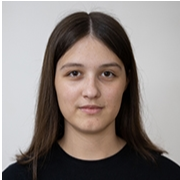
\includegraphics[width=3.5cm, height=3.5cm]{cover/A104437.png} & 
\includegraphics[width=3.5cm, height=3.5cm]{cover/A104263.png} & 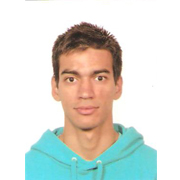
\includegraphics[width=3.5cm, height=3.5cm]{cover/A76350.jpg} \\
    Ana Sá Oliveira & Inês Silva Marques & José Rafael de \\
    (a104437) & (a104263) & Oliveira Vilas Boas \\
    && (a76350) \\
    \end{tabular}
    \\
    
\includegraphics[width=4cm, height=4cm]{cover/Bugbusters.png}
    \\
}
\date{\today}

\begin{document}
\maketitle
\begin{abstract}
    Este projeto teve como objetivo o desenvolvimento de um compilador para a linguagem Pascal Standard. O compilador foi construído em várias etapas, começando pela análise léxica, utilizando a biblioteca ply.lex para transformar o código-fonte em uma sequência de tokens. A seguir, foi implementada a análise sintática com ply.yacc, validando a estrutura do programa com base na gramática da linguagem.
    A partir do código reconhecido, foi construída uma árvore sintática abstrata (AST), que representa de forma estruturada os elementos do programa. Com base nessa AST, foi realizada a análise semântica, incluindo verificação de declarações, tipos e coerência do código.
    Na etapa de geração de código, adotámos uma abordagem de tradução dirigida pela sintaxe, convertendo a AST diretamente em código para uma máquina virtual disponibilizada no projeto.

    MELHORA

\end{abstract}

\tableofcontents
%\listoffigures
%\listoftables

\chapter{Introdução}
%\section{}
%\subsection{}
\textcolor{red}{\textbf{TODO}}

\chapter{Análise Léxica}

\textcolor{red}{\textbf{TODO}}

\chapter{Análise Sintática}

\section{Gramática}

\begin{tabbing}
\hspace{1.3cm}\= \hspace{11cm}\= \kill
\textbf{p0:}  \> S' \(\to\) program \\
\textbf{p1:}  \> program \(\to\) PROGRAM ID ; declarations code\_block . \\
\textbf{p2:}  \> program \(\to\) declarations code\_block . \\
\textbf{p3:}  \> declarations \(\to\) declarations declaration \\
\textbf{p4:}  \> declarations \(\to\) \(\epsilon\) \\
\textbf{p5:}  \> declaration \(\to\) variables\_declaration \\
\textbf{p6:}  \> declaration \(\to\) function \\
\textbf{p7:}  \> declaration \(\to\) procedure \\
\textbf{p8:}  \> variables\_declaration \(\to\) VAR variables\_list \\
\textbf{p9:}  \> variables\_list \(\to\) variables\_list same\_type\_variables \\
\textbf{p10:} \> variables\_list \(\to\) same\_type\_variables \\
\textbf{p11:} \> same\_type\_variables \(\to\) id\_list : DATATYPE ; \\
\textbf{p12:} \> same\_type\_variables \(\to\) id\_list : ARRAY [ INT RANGE INT ] OF DATATYPE ; \\
\textbf{p13:} \> id\_list \(\to\) id\_list , ID \\
\textbf{p14:} \> id\_list \(\to\) ID \\
\textbf{p15:} \> var\_or\_not \(\to\) variables\_declaration \\
\textbf{p16:} \> var\_or\_not \(\to\) \(\epsilon\) \\
\textbf{p17:} \> function \(\to\) FUNCTION ID ( parameters ) : DATATYPE ; var\_or\_not code\_block ; \\
\textbf{p18:} \> procedure \(\to\) PROCEDURE ID ( parameters ) ; var\_or\_not code\_block ; \\
\textbf{p19:} \> parameters \(\to\) parameter\_list \\
\textbf{p20:} \> parameters \(\to\) \(\epsilon\) \\
\textbf{p21:} \> parameter\_list \(\to\) parameter\_list ; parameter \\
\textbf{p22:} \> parameter\_list \(\to\) parameter \\
\textbf{p23:} \> parameter \(\to\) VAR\_opt id\_list : DATATYPE \\
\textbf{p24:} \> VAR\_opt \(\to\) VAR \\
\textbf{p25:} \> VAR\_opt \(\to\) \(\epsilon\) \\
\textbf{p26:} \> code\_block \(\to\) BEGIN algorithm END \\
\textbf{p27:} \> algorithm \(\to\) algorithm ; statement \\
\textbf{p28:} \> algorithm \(\to\) statement \\
\textbf{p29:} \> statement \(\to\) assignment \\
\textbf{p30:} \> statement \(\to\) func\_call \\
\textbf{p31:} \> statement \(\to\) loop \\
\textbf{p32:} \> statement \(\to\) code\_block \\
\textbf{p33:} \> statement \(\to\) if \\
\textbf{p34:} \> statement \(\to\) else \\
\textbf{p35:} \> statement \(\to\) \(\epsilon\) \\
\textbf{p36:} \> if \(\to\) IF cond THEN statement \\
\textbf{p37:} \> else \(\to\) IF cond THEN statement ELSE statement \\
\textbf{p38:} \> assignment \(\to\) ID ASSIGNMENT cond \\
\textbf{p39:} \> loop \(\to\) for \\
\textbf{p40:} \> loop \(\to\) while \\
\textbf{p41:} \> for \(\to\) FOR for\_cond DO statement \\
\textbf{p42:} \> for\_cond \(\to\) assignment TO cond \\
\textbf{p43:} \> for\_cond \(\to\) assignment DOWNTO cond \\
\textbf{p44:} \> while \(\to\) WHILE cond DO statement \\
\textbf{p45:} \> cond \(\to\) expr \\
\textbf{p46:} \> cond \(\to\) expr op\_rel expr \\
\textbf{p47:} \> op\_rel \(\to\) = \\
\textbf{p48:} \> op\_rel \(\to\) NOT\_EQUAL \\
\textbf{p49:} \> op\_rel \(\to\) < \\
\textbf{p50:} \> op\_rel \(\to\) LESS\_EQUAL \\
\textbf{p51:} \> op\_rel \(\to\) > \\
\textbf{p52:} \> op\_rel \(\to\) GREATER\_EQUAL \\
\textbf{p53:} \> expr \(\to\) termo \\
\textbf{p54:} \> expr \(\to\) expr op\_ad termo \\
\textbf{p55:} \> termo \(\to\) fator \\
\textbf{p56:} \> termo \(\to\) termo op\_mul fator \\
\textbf{p57:} \> op\_ad \(\to\) + \\
\textbf{p58:} \> op\_ad \(\to\) - \\
\textbf{p59:} \> op\_ad \(\to\) OR \\
\textbf{p60:} \> op\_mul \(\to\) * \\
\textbf{p61:} \> op\_mul \(\to\) / \\
\textbf{p62:} \> op\_mul \(\to\) AND \\
\textbf{p63:} \> op\_mul \(\to\) MOD \\
\textbf{p64:} \> op\_mul \(\to\) DIV \\
\textbf{p65:} \> fator \(\to\) value \\
\textbf{p66:} \> fator \(\to\) ( cond ) \\
\textbf{p67:} \> fator \(\to\) NOT fator \\
\textbf{p68:} \> value \(\to\) ID \\
\textbf{p69:} \> value \(\to\) INT \\
\textbf{p70:} \> value \(\to\) REAL \\
\textbf{p71:} \> value \(\to\) STRING \\
\textbf{p72:} \> value \(\to\) BOOL \\
\textbf{p73:} \> value \(\to\) ID [ INT ] \\
\textbf{p74:} \> value \(\to\) ID [ ID ] \\
\textbf{p75:} \> value \(\to\) func\_call \\
\textbf{p76:} \> func\_call \(\to\) ID ( args ) \\
\textbf{p77:} \> args \(\to\) elems \\
\textbf{p78:} \> args \(\to\) \(\epsilon\) \\
\textbf{p79:} \> elems \(\to\) elems , cond \\
\textbf{p80:} \> elems \(\to\) cond \\
\end{tabbing}

\textcolor{red}{\textbf{TODO}}

\chapter{Análise Semântica}

\textcolor{red}{\textbf{TODO}}

\chapter{Geração de Código}

\textcolor{red}{\textbf{TODO}}

\chapter{Otimização de Código}

\textcolor{red}{\textbf{TODO}}

\chapter{Testes}

\textcolor{red}{\textbf{TODO}}

\chapter{Conclusão}

\textcolor{red}{\textbf{TODO}}

\end{document}